\documentclass[fleqn]{article}

\usepackage{listings}
\usepackage{diagbox}
\usepackage[german]{babel}
\usepackage[T1]{fontenc}
\usepackage[latin1]{inputenc}
\usepackage{titlesec}
\usepackage{geometry}
\usepackage{qtree}
\usepackage{tikz}
\usepackage{amsmath}
\usepackage{amssymb}
\setcounter{secnumdepth}{0}
\usetikzlibrary{positioning}
\geometry{top=2.5cm, bottom=2.5cm}
\lstset{
 columns=fixed,       
 numbers=left,                                        % 在左侧显示行号
 numberstyle=\tiny\color{gray},                       % 设定行号格式
 frame=none,                                          % 不显示背景边框
 backgroundcolor=\color[RGB]{245,245,244},            % 设定背景颜色
 keywordstyle=\color[RGB]{40,40,255},                 % 设定关键字颜色
 numberstyle=\footnotesize\color{darkgray},           
 commentstyle=\it\color[RGB]{0,96,96},                % 设置代码注释的格式
 stringstyle=\rmfamily\slshape\color[RGB]{128,0,0},   % 设置字符串格式
 showstringspaces=false,                              % 不显示字符串中的空格
 language=c++,                                        % 设置语言
 breaklines,                                          % 自动换行
}

\title{TU Chemnitz \\ Praktikum Grundlagen Technische Informatik \\ Versuch Sequ1}

\author{Gruppe 5 - Team 5: \\ Dongze Yang \\Xiangyu Tong \\ Treshchun Kateryna}

\begin{document}

\maketitle



\newpagestyle{main}{
    \sethead{}{}{Grupe 5 - Team 5}
    \setfoot{}{\thepage}{}
    \headrule
    \footrule
}
\pagestyle{main}
%\section{Aufgabe}

\section{3.1 Untersuchung zweier statischer D-FF}

$$Q'_1 = \overline{\overline{CD + \bar{\bar{\bar{\bar{\bar{C}}}}}Q_1}} = CD+\bar{C}Q_1$$
$$Q'_2 = \overline{\overline{\overline{C}Q_2+\bar{\bar{\bar{\bar{C}}}}D}} = CD + \bar{C}Q_2$$


% \textbf{Wahrheitstabelle:}

% \begin{center}
% \begin{tabular}{cccc|cc}
%     $C$ & $D$ & $Q_1$ & $Q'_1$ & $Q_2$ & $Q'_2$\\
%     \hline
%     $\times$ & $\times$ & $\times$ & $Q_1$ & $\times$ & $Q_2$\\
%     0&0&0&0&0&0\\
%     0&0&1&1&1&1\\
%     0&1&0&0&0&0\\
%     0&1&1&1&1&1\\
%     1&0&0&0&0&0\\
%     1&0&1&0&1&0\\
%     1&1&0&1&0&1\\
%     1&1&1&1&1&1
% \end{tabular}
% \end{center}

\subsection{Simulativ:}

\begin{figure}[!hb]
    \centering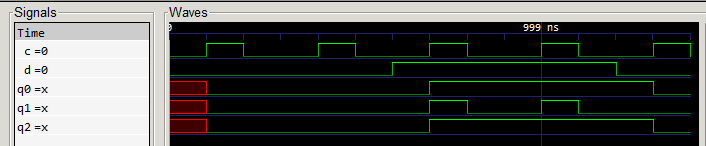
\includegraphics[width=6in]{ohne.png}
    \caption{Simulation ohne Zeitverzögerung}

    \centering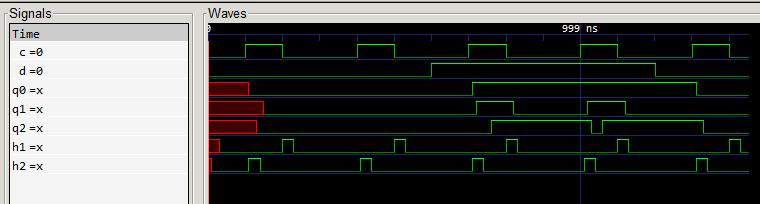
\includegraphics[width=6in]{mit.png}
    \caption{Simulation mit Zeitverzögerung}
\end{figure}

\textbf{Dabei sollte folgende Frage beantwortet werden: Warum ist Flipflop 1, obwohl es augenscheinlich die gleiche charakteristische Gleichung wie Flipflop 2 besitzt, als Flipflop ungeeignet?}

An Position 800ns erkennt man recht gut das Problem. 
Hier kommt es durch die unterschiedliche Anzahl der vorgeschaltenen Gatter zu einer zeitlichen Differenz zwischen dem Signal $C$ und $\overline{C}$. 
Im ersten Flipflop liegt nun bei $C$ und $\overline{C}$ eine 0 an, 
weshalb $Q_1$ seinen aktuellen Zustand verliert und auf 0 wechselt. 
Beim 2. Flipflop hingegen liegt bei $C$ und $\overline{C}$ eine 1 an. 
Ähnlich sieht es bei 1us am 2. Flipflop aus. 
Beim Wechsel von $C$ von 0 auf 1 wechselt zuerst $\overline{C}$ von 1 auf 0, 
setzt damit $Q_2$ auf 0, bevor $C$ auf 1 wechselt und somit den Dateneingang übernimmt und $Q_2$ wieder auf 1 springt. 
\\
\subsection{VHDL-Strukturbeschreibung}

\begin{lstlisting}
library ieee; 
use ieee.std_logic_1164.all; 
use work.pack_2.all;

entity uut is 
    port (EE_X : in X01_vector (7 downto 0); 
EE_Y : out X01_vector (23 downto 16));
end uut; 

architecture structure of uut is

component sn7404 is -- 1/6 SN7404 
    port (x : in X01; 
        y : out X01); 
end component;

component sn7450 is -- 1/2 SN7450 
    port (x11 ,x12 ,x21 ,x22 : in X01; y : out X01); 
end component;

alias c1 : X01 is EE_X(0); 
alias d1 : X01 is EE_X(1); 
alias q11 : X01 is EE_Y(16); 
alias q12 : X01 is EE_Y(17); 

signal c,d : X01; 
signal s11 ,s12 ,s13 ,s14 ,s15 ,s21 ,s22 ,s23 ,s24 : X01; 

signal n1,n2 : x01; 
signal h1,h2 : x01; -- Hilfsausgänge der D-Flipflops

begin 

-- D-Flipflop1 
d11: sn7404 port map (x=>c1, y=>s11); 
d12: sn7404 port map (x=>s11, y=>s12); 
d13: sn7404 port map (x=>s12, y=>s13); 
d14: sn7404 port map (x=>s13, y=>s14);
d15: sn7404 port map (x=>s14, y=>s15);  
d16: sn7450 port map (x11=>h1, x12=>s15, x21=>c1, x22=>d1, y=>n1);
d17: sn7404 port map (x=>n1, y=>h1);
q11 <= h1;  

-- D-Flipflop2 
d21: sn7404 port map (x=>c1, y=>s21); 
d22: sn7404 port map (x=>s21, y=>s22); 
d23: sn7404 port map (x=>s22, y=>s23); 
d24: sn7404 port map (x=>s23, y=>s24); 
d25: sn7450 port map (x11=>h2, x12=>s21, x21=>s24, x22=>d1, y=>n2);
d26: sn7404 port map (x=>n2, y=>h2); 
q12 <= h2;
end structure;
\end{lstlisting}

\subsection{Binäre Stimulusfolge}
\begin{lstlisting}
stimmap dbb2_08 --------|--------  DUMMY
stimmap dbb2_08 00------|XX-----
stimmap dbb2_08 10------|00-----
stimmap dbb2_08 00------|00-----
stimmap dbb2_08 00------|00-----
stimmap dbb2_08 10------|00-----
stimmap dbb2_08 00------|00-----
stimmap dbb2_08 01------|00-----
stimmap dbb2_08 11------|11-----
stimmap dbb2_08 01------|11-----
stimmap dbb2_08 01------|11-----
stimmap dbb2_08 11------|11-----
stimmap dbb2_08 01------|11-----
stimmap dbb2_08 00------|11-----
stimmap dbb2_08 10------|00-----
stimmap dbb2_08 00------|00-----
\end{lstlisting}

\subsection{Ternäre Stimulusfolge}
\begin{lstlisting}
stimmap dbb2_08 00------|XX-----
stimmap dbb2_08 X0------|XX-----
stimmap dbb2_08 10------|00-----
stimmap dbb2_08 X0------|00-----
stimmap dbb2_08 00------|00-----
stimmap dbb2_08 00------|00-----
stimmap dbb2_08 X0------|00-----
stimmap dbb2_08 10------|00-----
stimmap dbb2_08 X0------|00-----
stimmap dbb2_08 00------|00-----
stimmap dbb2_08 0X------|00-----
stimmap dbb2_08 01------|00-----
stimmap dbb2_08 X1------|00-----
stimmap dbb2_08 11------|11-----
stimmap dbb2_08 X1------|11-----
stimmap dbb2_08 01------|11-----
stimmap dbb2_08 01------|11-----
stimmap dbb2_08 X1------|11-----
stimmap dbb2_08 11------|11-----
stimmap dbb2_08 X1------|11-----
stimmap dbb2_08 01------|11-----
stimmap dbb2_08 0X------|11-----
stimmap dbb2_08 00------|11-----
stimmap dbb2_08 X0------|11-----
stimmap dbb2_08 10------|00-----
stimmap dbb2_08 X0------|00-----
stimmap dbb2_08 00------|00-----
\end{lstlisting}

\section{3.2 FF-Substitution}

$JK\rightarrow D$ \qquad \qquad \qquad \qquad \qquad \qquad \qquad KV-Diagramm:


\begin{tabular}{cc|cc|c}
    $J$&$K$&$Q^n$&$Q^{n+1}$&$D$\\
    \hline
    0&0&0&0&0\\
    0&0&1&1&1\\
    0&1&0&0&0\\
    0&1&1&0&0\\
    1&0&0&1&1\\
    1&0&1&1&1\\
    1&1&0&1&1\\
    1&1&1&0&0
\end{tabular} \qquad \qquad \qquad \qquad
\begin{tabular}{cc|cc}
    &&$Q$\\
    \hline
    $J$&$K$&0&1\\
    \hline
    0&0&0&1\\
    0&1&0&0\\
    1&1&1&0\\
    1&0&1&1
\end{tabular}

$$DFF: Q^{n+1} = D$$

$$JKFF: Q^{n+1} = J\overline{Q^{n}} + \overline{K}Q^{n}$$

$$\Rightarrow D = J\overline{Q^{n}} + \overline{K}Q^{n}$$

$$C_{JK} = \overline{C}$$

\subsection{Schaltplan}

\begin{figure}[!hb]
    \centering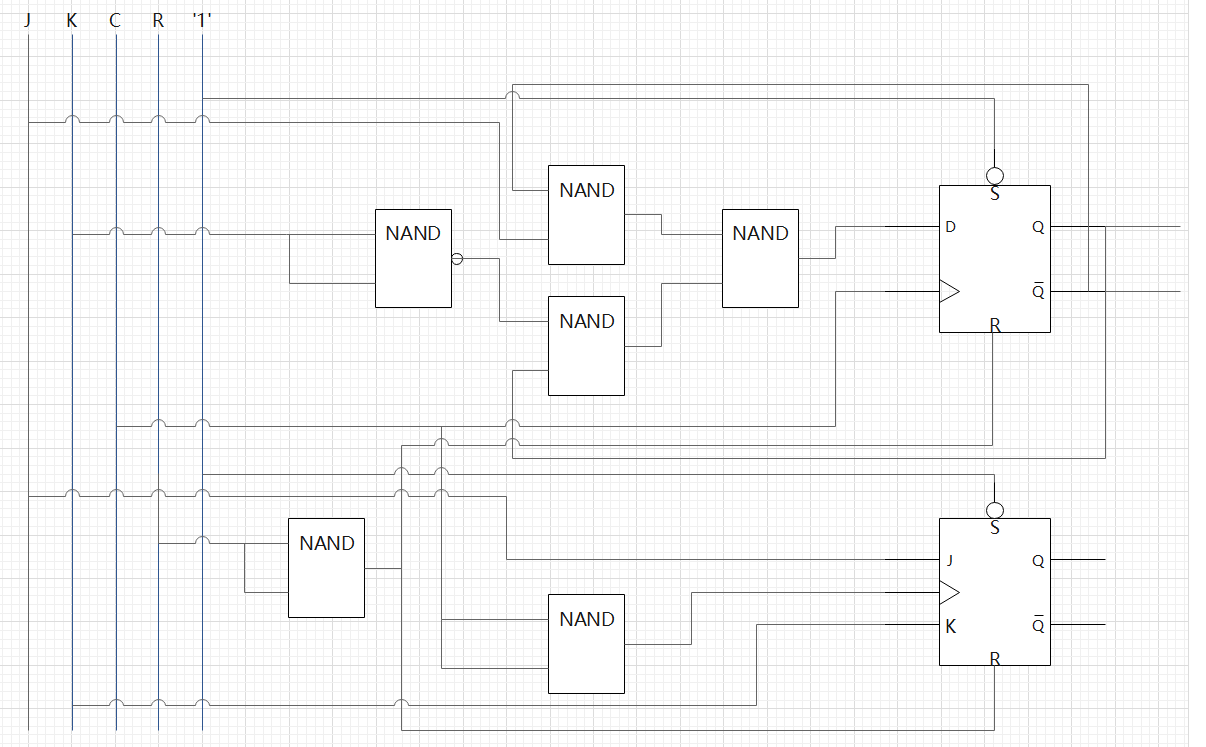
\includegraphics[width=6in]{bild1.png}
\end{figure}

\subsection{VHDL-Strukturbeschreibung}
\begin{lstlisting}
library ieee; 
use ieee.std_logic_1164.all; 
use work.pack_2.all; 
entity uut is 
    port ( EE_X : in X01_vector (7 downto 0);
            EE_Y : out X01_vector (23 downto 16));
end uut; 
architecture structure of uut is 
    component sn7400 is --2xSN7400NAND 
        port ( x : in X01_vector (1 to 2); y : out X01 ); 
    end component; 

    component sn7472 is --SN7472 JKFF
        port ( s_b , r_b , c : in X01; 
                j , k : in X01_vector (1 to 3); 
                q , q_b : out X01 ); 
    end component;

    component sn7474 is --SN7474 D-FF 
        port ( s_b , r_b , c , d : in X01;
                q , q_b : out X01 ); 
    end component; 
    alias j : X01 is EE_X(4); 
    alias k : X01 is EE_X(5);
    alias c : X01 is EE_X(6); 
    alias r : X01 is EE_X(7); 
    alias q1_out : X01 is EE_Y (20); 
    alias q2_out : X01 is EE_Y (21); 
    signal nk , q1 , nq1 , l6_13 , l8_12 , l11_d : X01; --D-FF 
    signal nc , q2 , nq2 : X01; --JKFF 
begin 

    NOTK: sn7400 port map (x(1)=>k , x(2)=>k , y=>nk); 
    NAND1: sn7400 port map (x(1)=>nq1 , x(2)=>j , y=>l6_13); 
    NAND2: sn7400 port map (x(1)=>nk , x(2)=>q1 , y=>l8_12); 
    NAND3: sn7400 port map (x(1)=>l6_13, x(2)=>l8_12, y=>l11_d); 
    D_FF: sn7474 port map (s_b=>'1', r_b=>r, c=>c, d=>l11_d, q=>q1, q_b=>nq1); 

    NOTC: sn7400 port map ( x(1)=>c , x(2)=>c , y=>nc );
    JK_FF: sn7472 port map ( s_b=>'1', r_b=>r , c=>nc , j(1)=>'1', j(2)=>j , j(3)=>'1', 
                                k(1)=>'1', k(2)=>k , k(3)=>'1', q=>q2 , q_b=>nq2 );

    q1_out<=q1; 
    q2_out<=q2; 
end structure;
\end{lstlisting}

\subsection{Stimulusfolgen für dynamisches JKFF}

\subsubsection{Binäre Stimulusfolge}
\begin{lstlisting}
stimmap dbb2_08 ----0001|----XX--
stimmap dbb2_08 ----0000|----00--
stimmap dbb2_08 ----0001|----00--
stimmap dbb2_08 ----0001|----00--
stimmap dbb2_08 ----0011|----00--
stimmap dbb2_08 ----0001|----00--
stimmap dbb2_08 ----0101|----00--
stimmap dbb2_08 ----0111|----00--
stimmap dbb2_08 ----0101|----00--
stimmap dbb2_08 ----1001|----00--
stimmap dbb2_08 ----1011|----11--
stimmap dbb2_08 ----1001|----11--
stimmap dbb2_08 ----0001|----11--
stimmap dbb2_08 ----0011|----11--
stimmap dbb2_08 ----0001|----11--
stimmap dbb2_08 ----1001|----11--
stimmap dbb2_08 ----1011|----11--
stimmap dbb2_08 ----1001|----11--
stimmap dbb2_08 ----0101|----11--
stimmap dbb2_08 ----0111|----00--
stimmap dbb2_08 ----0101|----00--
stimmap dbb2_08 ----1101|----00--
stimmap dbb2_08 ----1111|----11--
stimmap dbb2_08 ----1101|----11--
stimmap dbb2_08 ----1101|----11--
stimmap dbb2_08 ----1111|----00--
stimmap dbb2_08 ----1101|----00--
\end{lstlisting}

\subsubsection{Ternäre Stimulusfolge}
\begin{lstlisting}
stimmap dbb2_08 ----0001|----XX--
stimmap dbb2_08 ----000X|--------
stimmap dbb2_08 ----0000|----00--
stimmap dbb2_08 ----000X|--------
stimmap dbb2_08 ----0001|----00--
stimmap dbb2_08 ----0001|----00--
stimmap dbb2_08 ----0011|----00--
stimmap dbb2_08 ----0001|----00--
stimmap dbb2_08 ----0X01|--------
stimmap dbb2_08 ----0101|----00--
stimmap dbb2_08 ----0111|----00--
stimmap dbb2_08 ----0101|----00--
stimmap dbb2_08 ----XX01|--------
stimmap dbb2_08 ----1001|----00--
stimmap dbb2_08 ----1011|----11--
stimmap dbb2_08 ----1001|----11--
stimmap dbb2_08 ----X001|--------
stimmap dbb2_08 ----0001|----11--
stimmap dbb2_08 ----0011|----11--
stimmap dbb2_08 ----0001|----11--
stimmap dbb2_08 ----X001|--------
stimmap dbb2_08 ----1001|----11--
stimmap dbb2_08 ----1011|----11--
stimmap dbb2_08 ----1001|----11--
stimmap dbb2_08 ----XX01|--------
stimmap dbb2_08 ----0101|----11--
stimmap dbb2_08 ----0111|----00--
stimmap dbb2_08 ----0101|----00--
stimmap dbb2_08 ----X101|--------
stimmap dbb2_08 ----1101|----00--
stimmap dbb2_08 ----1111|----11--
stimmap dbb2_08 ----1101|----11--
stimmap dbb2_08 ----1101|----11--
stimmap dbb2_08 ----1111|----00--
stimmap dbb2_08 ----1101|----00--
\end{lstlisting}


\subsection{Stimulusfolgen für JKMSFF}

\subsubsection{Binäre Stimulusfolge}
\begin{lstlisting}
stimmap dbb2_08 ----0001|----XX-- stat Reset
stimmap dbb2_08 ----0000|----00-- (Zustand 00)
stimmap dbb2_08 ----0001|----00-- speichern
stimmap dbb2_08 ----0000|----00-- Res(Reset aus 00)
stimmap dbb2_08 ----0001|----00-- speichern
stimmap dbb2_08 ----0101|----00-- speichern
stimmap dbb2_08 ----0111|----00-- speichern
stimmap dbb2_08 ----1111|----00-- speichern
stimmap dbb2_08 ----1011|----00-- speichern
stimmap dbb2_08 ----0011|----00-- speichern
stimmap dbb2_08 ----0001|----00-- speichern
stimmap dbb2_08 ----0001|----00-- speichern
stimmap dbb2_08 ----1001|----00-- (Zustand 10, Kante 1)
stimmap dbb2_08 ----1101|----00-- speichern
stimmap dbb2_08 ----0101|----00-- speichern
stimmap dbb2_08 ----0001|----00-- speichern
stimmap dbb2_08 ----1001|----00-- speichern
stimmap dbb2_08 ----0001|----00-- speichern
stimmap dbb2_08 ----0000|----00-- Res(Reset aus 10)
stimmap dbb2_08 ----0001|----00-- speichern
stimmap dbb2_08 ----1101|----00-- (Zustand 10 , Kante 2)
stimmap dbb2_08 ----0001|----00-- speichern
stimmap dbb2_08 ----0001|----00-- speichern
stimmap dbb2_08 ----0011|----01-- (Zustand 11 , Kante 1)
stimmap dbb2_08 ----0011|----01-- speichern
stimmap dbb2_08 ----0111|----01-- speichern
stimmap dbb2_08 ----1111|----01-- speichern
stimmap dbb2_08 ----1011|----01-- speichern
stimmap dbb2_08 ----1001|----01-- speichern
stimmap dbb2_08 ----0001|----01-- speichern
stimmap dbb2_08 ----0000|----00-- Reset (Reset aus 11)
stimmap dbb2_08 ----0001|----00-- speichern
stimmap dbb2_08 ----1001|----00-- (Zustand 10 , Kante 1)
stimmap dbb2_08 ----0001|----00-- speichern
stimmap dbb2_08 ----0101|----00-- speichern
stimmap dbb2_08 ----0111|----01-- (Zustand 11 , Kante 2)
stimmap dbb2_08 ----0101|----01-- (Zustand 01 , Kante 1)
stimmap dbb2_08 ----1101|----01-- speichern
stimmap dbb2_08 ----0101|----01-- speichern
stimmap dbb2_08 ----0001|----01-- speichern
stimmap dbb2_08 ----1001|----01-- speichern
stimmap dbb2_08 ----0001|----01-- speichern
stimmap dbb2_08 ----0000|----00-- Reset (Reset aus 01)
stimmap dbb2_08 ----0001|----00-- speichern
stimmap dbb2_08 ----1001|----00-- (Zustand 10 , Kante 1)
stimmap dbb2_08 ----1011|----11-- (Zustand 11 , Kante 3)
stimmap dbb2_08 ----1001|----11-- speichern
stimmap dbb2_08 ----1101|----11-- (Zustand 01 , Kante 2)
stimmap dbb2_08 ----1101|----11-- speichern
stimmap dbb2_08 ----1111|----00-- (Zustand 00 , Kante 1)
stimmap dbb2_08 ----1101|----00-- (Zustand 10 , Kante 2)
stimmap dbb2_08 ----1001|----00-- speichern
stimmap dbb2_08 ----1011|----11-- (Zustand 11 , Kante 3)
stimmap dbb2_08 ----1001|----11-- speichern
stimmap dbb2_08 ----1101|----11-- (Zustand 10 , Kante 2)
stimmap dbb2_08 ----1001|----11-- speichern
stimmap dbb2_08 ----1011|----10-- (Zustand 00 , Kante 2)
stimmap dbb2_08 ----1001|----10-- (Zustand 10 , Kante 1)
stimmap dbb2_08 ----1101|----10-- speichern
stimmap dbb2_08 ----1111|----01-- (Zustand 11 , Kante 4)
stimmap dbb2_08 ----1101|----01-- (Zustand 01 , Kante 2)
stimmap dbb2_08 ----0101|----01-- speichern
stimmap dbb2_08 ----0111|----00-- (Zustand 00 , Kante 3)
stimmap dbb2_08 ----0101|----00-- speichern
stimmap dbb2_08 ----1101|----00-- (Zustand 10 , Kante 2)
stimmap dbb2_08 ----1111|----11-- (Zustand 11 , Kante 4)
stimmap dbb2_08 ----1101|----11-- (Zustand 01 , Kante 2)
stimmap dbb2_08 ----0001|----11-- speichern
stimmap dbb2_08 ----0011|----10-- (Zustand 00 , Kante 4)
stimmap dbb2_08 ----0001|----10-- speichern
\end{lstlisting}

\subsubsection{Ternäre Stimulusfolge}
\begin{lstlisting}
stimmap dbb2_08 ----0001|----XX--
stimmap dbb2_08 ----000X|--------
stimmap dbb2_08 ----0000|----00--
stimmap dbb2_08 ----000X|--------
stimmap dbb2_08 ----0001|----00--
stimmap dbb2_08 ----000X|--------
stimmap dbb2_08 ----0000|----00--
stimmap dbb2_08 ----000X|--------
stimmap dbb2_08 ----0001|----00--
stimmap dbb2_08 ----0X01|--------
stimmap dbb2_08 ----0101|----00--
stimmap dbb2_08 ----0111|----00--
stimmap dbb2_08 ----X111|--------
stimmap dbb2_08 ----1111|----00--
stimmap dbb2_08 ----1X11|--------
stimmap dbb2_08 ----1011|----00--
stimmap dbb2_08 ----X011|--------
stimmap dbb2_08 ----0011|----00--
stimmap dbb2_08 ----0001|----00--
stimmap dbb2_08 ----0001|----00--
stimmap dbb2_08 ----X001|--------
stimmap dbb2_08 ----1001|----00--
stimmap dbb2_08 ----1X01|--------
stimmap dbb2_08 ----1101|----00--
stimmap dbb2_08 ----X101|--------
stimmap dbb2_08 ----0101|----00--
stimmap dbb2_08 ----0X01|--------
stimmap dbb2_08 ----0001|----00--
stimmap dbb2_08 ----X001|--------
stimmap dbb2_08 ----1001|----00--
stimmap dbb2_08 ----X001|--------
stimmap dbb2_08 ----0001|----00--
stimmap dbb2_08 ----000X|--------
stimmap dbb2_08 ----0000|----00--
stimmap dbb2_08 ----000X|--------
stimmap dbb2_08 ----0001|----00--
stimmap dbb2_08 ----XX01|--------
stimmap dbb2_08 ----1101|----00--
stimmap dbb2_08 ----XX01|--------
stimmap dbb2_08 ----0001|----00--
stimmap dbb2_08 ----0011|----01--
stimmap dbb2_08 ----0011|----01--
stimmap dbb2_08 ----0X11|--------
stimmap dbb2_08 ----0111|----01--
stimmap dbb2_08 ----X111|--------
stimmap dbb2_08 ----1111|----01--
stimmap dbb2_08 ----1X11|--------
stimmap dbb2_08 ----1011|----01--
stimmap dbb2_08 ----1001|----01--
stimmap dbb2_08 ----X001|--------
stimmap dbb2_08 ----0001|----01--
stimmap dbb2_08 ----000X|--------
stimmap dbb2_08 ----0000|----00--
stimmap dbb2_08 ----000X|--------
stimmap dbb2_08 ----0001|----00--
stimmap dbb2_08 ----X001|--------
stimmap dbb2_08 ----1001|----00--
stimmap dbb2_08 ----X001|--------
stimmap dbb2_08 ----0001|----00--
stimmap dbb2_08 ----0X01|--------
stimmap dbb2_08 ----0101|----00--
stimmap dbb2_08 ----0111|----01--
stimmap dbb2_08 ----0101|----01--
stimmap dbb2_08 ----X101|--------
stimmap dbb2_08 ----1101|----01--
stimmap dbb2_08 ----X101|--------
stimmap dbb2_08 ----0101|----01--
stimmap dbb2_08 ----0X01|--------
stimmap dbb2_08 ----0001|----01--
stimmap dbb2_08 ----X001|--------
stimmap dbb2_08 ----1001|----01--
stimmap dbb2_08 ----X001|--------
stimmap dbb2_08 ----0001|----01--
stimmap dbb2_08 ----000X|--------
stimmap dbb2_08 ----0000|----00--
stimmap dbb2_08 ----000X|--------
stimmap dbb2_08 ----0001|----00--
stimmap dbb2_08 ----X001|--------
stimmap dbb2_08 ----1001|----00--
stimmap dbb2_08 ----1011|----11--
stimmap dbb2_08 ----1001|----11--
stimmap dbb2_08 ----1X01|--------
stimmap dbb2_08 ----1101|----11--
stimmap dbb2_08 ----1101|----11--
stimmap dbb2_08 ----1111|----00--
stimmap dbb2_08 ----1101|----00--
stimmap dbb2_08 ----1X01|--------
stimmap dbb2_08 ----1001|----00--
stimmap dbb2_08 ----1011|----11--
stimmap dbb2_08 ----1001|----11--
stimmap dbb2_08 ----1X01|--------
stimmap dbb2_08 ----1101|----11--
stimmap dbb2_08 ----1X01|--------
stimmap dbb2_08 ----1001|----11--
stimmap dbb2_08 ----1011|----10--
stimmap dbb2_08 ----1001|----10--
stimmap dbb2_08 ----1X01|--------
stimmap dbb2_08 ----1101|----10--
stimmap dbb2_08 ----1111|----01--
stimmap dbb2_08 ----1101|----01--
stimmap dbb2_08 ----X101|--------
stimmap dbb2_08 ----0101|----01--
stimmap dbb2_08 ----0111|----00--
stimmap dbb2_08 ----0101|----00--
stimmap dbb2_08 ----X101|--------
stimmap dbb2_08 ----1101|----00--
stimmap dbb2_08 ----1111|----11--
stimmap dbb2_08 ----1101|----11--
stimmap dbb2_08 ----XX01|--------
stimmap dbb2_08 ----0001|----11--
stimmap dbb2_08 ----0011|----10--
stimmap dbb2_08 ----0001|----10--
\end{lstlisting}

\end{document}